\documentclass[titlepage, 11pt]{article}
\usepackage[a4paper, total={6in, 9.5in}]{geometry}
\usepackage{graphicx}
\usepackage{amsmath,amsfonts,amssymb}
\usepackage{listings}
\usepackage{booktabs}
\usepackage[T1]{fontenc}
\usepackage{listings}
\usepackage{color}
\usepackage{minted}
\usepackage[colorlinks=true, linkcolor=blue, urlcolor=blue, citecolor=blue, pdfborder={0 0 255}]{hyperref}
\usepackage{colortbl}
\usepackage{url}
\usepackage{xcolor}
\usepackage{caption}
\usepackage{subcaption}
\usepackage{dirtytalk}
\usepackage[semicolon, round]{natbib}
\usepackage[ruled]{algorithm2e}
\captionsetup[table]{skip=10pt}
\renewcommand{\vec}[1]{\mathbf{#1}}
\SetKwComment{Comment}{$\triangleright$\ }{}
% \hypersetup{%
% 	colorlinks=true,
% 	linkcolor=blue,
% 	linkbordercolor={0 0 1}
% }

% \renewcommand\lstlistingname{Algorithm}
% \renewcommand\lstlistlistingname{Algorithms}
% \def\lstlistingautorefname{Alg.}

% \lstdefinestyle{Python}{
% 	language        = Python,
% 	frame           = lines, 
% 	basicstyle      = \footnotesize,
% 	keywordstyle    = \color{blue},
% 	stringstyle     = \color{green},
% 	commentstyle    = \color{red}\ttfamily
% }

% \setlength{\parindent}{0.0in}
% \setlength{\parskip}{0.05in}

\newcommand{\argmin}{\mathop{\mathrm{argmin}}}
\newcommand{\argmax}{\mathop{\mathrm{argmax}}}
\newcommand{\minimize}{\mathop{\mathrm{minimize}}}
\newcommand{\maximize}{\mathop{\mathrm{maximize}}}
\newcommand{\st}{\mathop{\mathrm{subject\,\,to}}}
\newcommand{\dist}{\mathop{\mathrm{dist}}}
\newcommand{\norm}[1]{\left\lVert#1\right\rVert}
\renewcommand{\vec}[1]{\mathbf{#1}}

\def\R{\mathbb{R}}
\def\E{\mathbb{E}}
\def\P{\mathbb{P}}
\def\S{\mathbb{S}}
\def\Cov{\mathrm{Cov}}
\def\Var{\mathrm{Var}}
\def\half{\frac{1}{2}}
\def\quat{\frac{1}{4}}
\def\sign{\mathrm{sign}}
\def\supp{\mathrm{supp}}
\def\th{\mathrm{th}}
\def\tr{\mathrm{tr}}
\def\dim{\mathrm{dim}}
\def\dom{\mathrm{dom}}

\title{
{EE1103: Numerical Methods} \\~\\
{\vlarge Programming Assignment {\#} 5}\\
}\author{ANIRUDH B S, EE21B019\\
Collaborators: & AMIZHTHNI P R K, EE21B015
 & ANKITA HARSHA MURTHY, EE21B020}
\date{\today}

\begin{document}
\maketitle

\setcounter{page}{0}
\tableofcontents
\listoffigures
\listoftables
\newpage

\section{Problem 1}
Use least-squares regression to fit a straight line to the data given. \\
Along with the slope and intercept, compute the standard error of the estimate and the correlation coefficient.\\ Plot the data as discrete points and
the regression line (as a continuous line) in the same set of axes. \\ If someone made an additional measurement of
x = 10, y = 10, would you suspect, based on a visual assessment
and the standard error, that the measurement was valid or faulty?
Justify your conclusion.
\begin{table}[h!]
\begin{center}
    \label{tab:table1}
    \begin{tabular}{|l|l|l|l|l|l|l|l|l|l|l|l|}
    \hline
      x & 6 & 7 & 11 & 15 & 17 & 21 & 23 & 29 & 29 & 37 & 39\\
      \hline
      y & 29 & 21 & 29 & 14 & 21 & 15 & 7 & 7 & 13 & 0 & 3 \\
      \hline
     
    \end{tabular}
\end{center}
\end{table}

\subsection{Approach}

In this problem, I shall use the Least-Square Regression to find out the best-fit straight line for a given set of data points. 

%%%%%%%%%%%%%%%%%%%%%%%%%%%%%%%%%%%%%%%%%%%%%%%%%%%%%%

\subsection{Algorithm}
In this section,I shall present the pseudocode/flowchart of the algorithm used to solve the problem.

The pseudocode for the summation is provided in Algorithm~\ref{alg1}.
\begin{center}
\begin{algorithm}[H]\label{alg1}

\SetAlgoLined
{
n $\gets$ 11 \\
x $\gets$ [$x_0,x_1,x_2.....x_{10}$] \\
y $\gets$ [$y_0,y_1,y_2.....y_{10}$] \\
$s$ $\gets$ n \\
$s_x$ $\gets$ 0 \\ 
$s_y$ $\gets$ 0 \\ 
$s_{xy}$ $\gets$ 0 \\ 
$s_{xx}$ $\gets$ 0 \\ 
$s_t$ $\gets$ 0 \\
$s_r$ $\gets$ 0 \\
\For {$i=0$ to n-1}{
  $s_x$ $\gets$ $s_x + x_i$ \\ 
  $s_y$ $\gets$ $s_y + y_i$ \\
  $s_{xy}$ $\gets$ $s_{xy} + x_iy_i$ \\
  $s_{xx}$ $\gets$ $s_{xx} + x_ix_i$ \\
}
A $\gets$
$\begin{pmatrix}
s & s_x\\
s_x & s_{xx}
\end{pmatrix}$ \\
B $\gets$
$\begin{pmatrix}
s_y \\
s_{xy}
\end{pmatrix}$ \\
X $\gets$
$\begin{pmatrix}
a_0 \\
a_1
\end{pmatrix}$ \\
Solve AX = B using Gauss Elimination \textbf{Assignment 4}\\
mean $\gets$ $\frac{s_y}{n}$ \\
\For{$i=0$ to n-1}{
   $s_r$ $\gets$ $s_r$ + $(y_i-a_0-a_1x_i)^2$ \\
   $s_t$ $\gets$ $s_t$ + $(y_i-mean)$ 
}
$\sigma$ $\gets$ $\sqrt{\frac{s_r}{n-2}}$\\
$r^2$ $\gets$ $\frac{s_t-s_r}{s_t}$\\
$r$ $\gets$ $\sqrt{\frac{s_t-s_r}{s_t}}$\\
}
 \caption{Least Square Regression}
\end{algorithm}    
\end{center}

%%%%%%%%%%%%%%%%%%%%%%%%%%%%%%%%%%%%%%%%%%%%%%%%%%%%%%
\subsection{Results}

In this section, I shall plot the graphs that provide an overview of my findings during this problem. 

I shall plot the graphs showing the best fit line for a given set of data points and also plot the data points given as discrete points  in Figure~\ref{fig:q11}. The results are also summarized below. 

As seen, the point (10,10) does not lie on the best fit line and is probable that the reading (10,10) may be erroneous. 

The equation of line obtained using linear regression is 
\begin{equation}
    y = 31.058898 - 0.780547 x
\end{equation}
At x = 10, we obtain y = 23.253433 which is clearly off y = 10. 
\begin{itemize}
\item [1] The value of the $S_r$ = 180.335835 
\item [2] The value of the coefficient of determination $r^2$ = 0.812682 
\item [3] The value of the coefficient of correlation $r$ = 0.901489
\item [4] The standard deviation or standard error of estimate is $s_{y/x}$ = 4.476306 
\end{itemize}
\begin{figure}[!tbh]
  	\centering
  	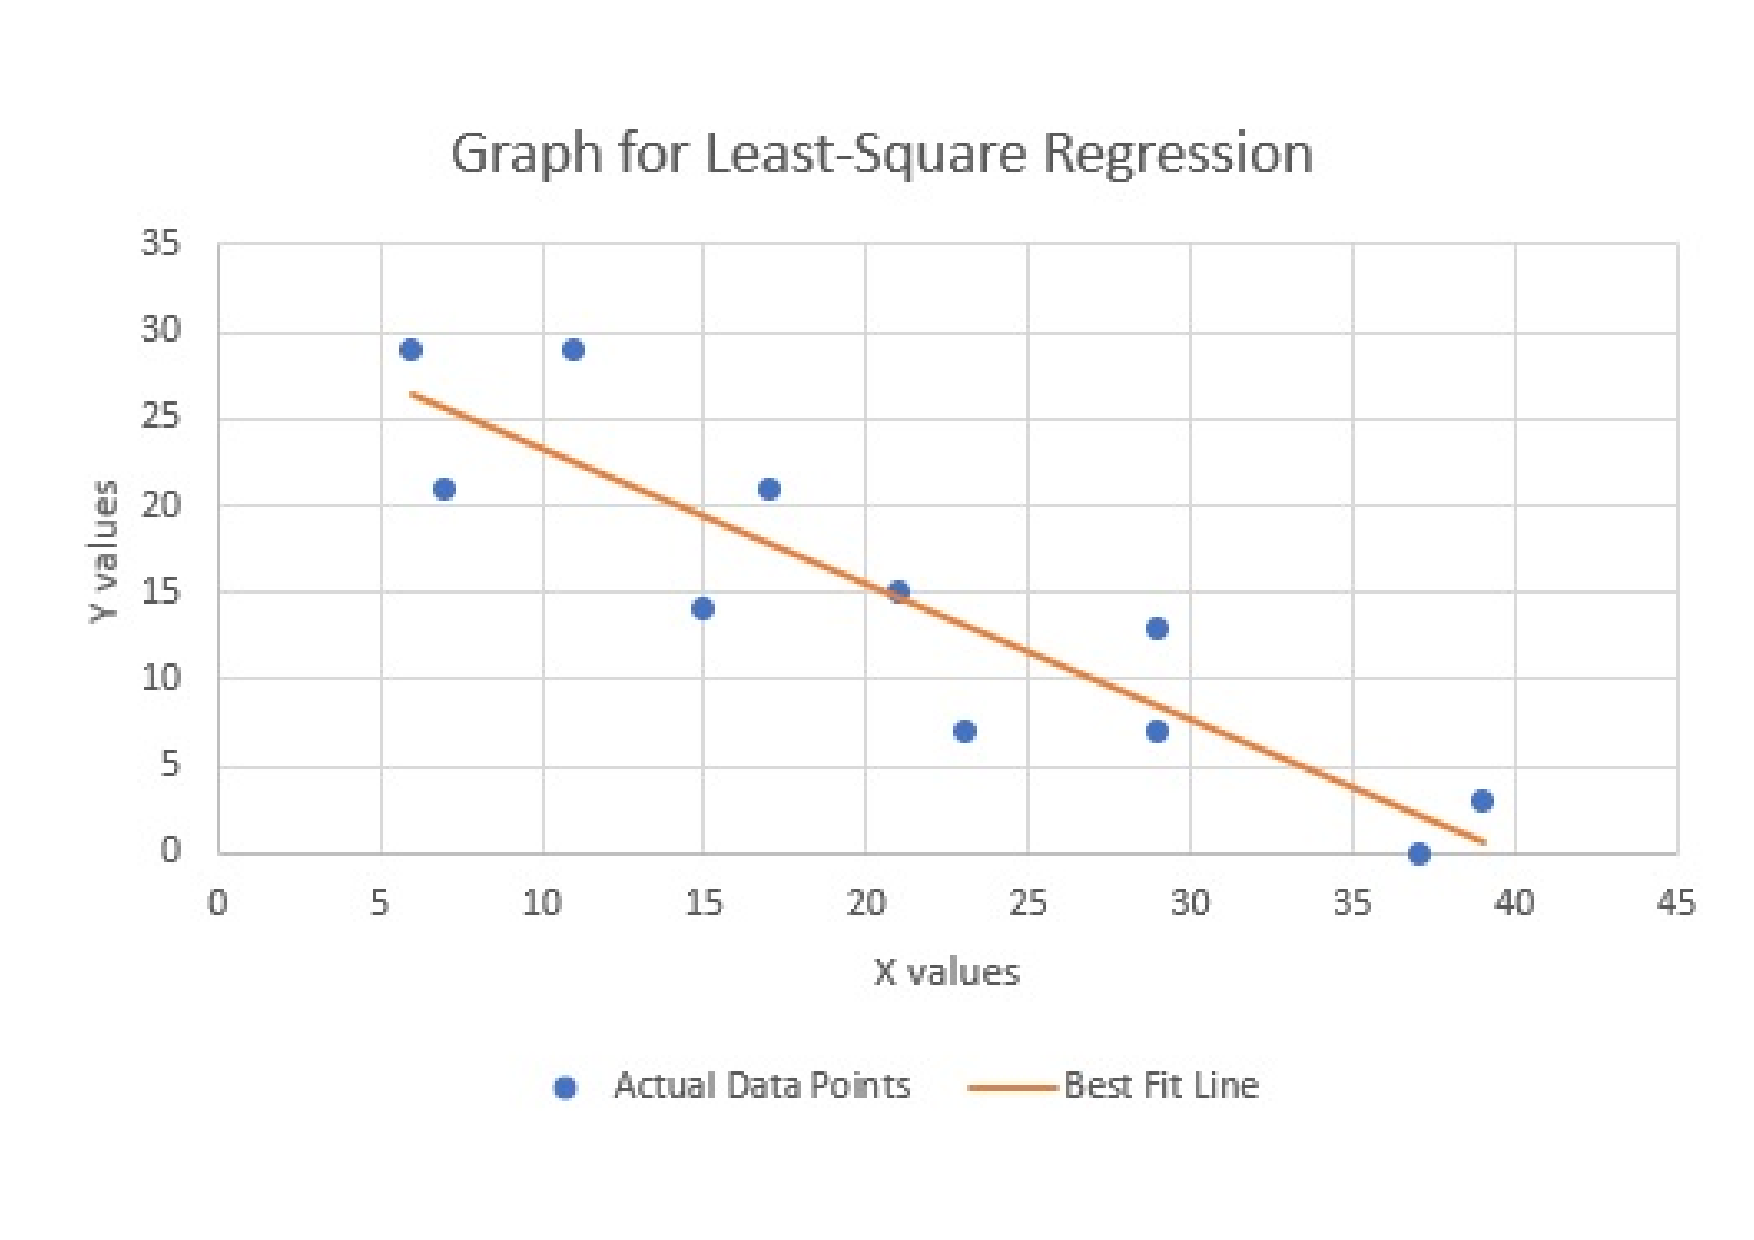
\includegraphics[width=0.9\textwidth]{A5P1Graph.pdf} 
  	\caption{Best Fit Straight Line obtained using Least Square Regression.}
  	\label{fig:q11} 
\end{figure}

%%%%%%%%%%%%%%%%%%%%%%%%%%%%%%%%%%%%%%%%%%%%%%%%%%%%%%

\subsection{Inferences}
I deduce the following inferences in this experiment:
\begin{itemize}
    \item [1] The value of the coefficient of determination $r^2$ is 0.812682 which is quite far off from 1 which denotes an ideal fit, thus, the linear fit is far from an ideal fit. 
    \item [2] Moreover, it can be seen clearly that the best fit straight line seldom passes through any of the given data points. Thus, the words \textbf{best fit} seems contradicting. 
    \item [3] This however, cannot be disregarded as not the best fit line as the algorithm devised by us works on minimizing the sum of squares of error terms. In most situations, this algorithm does generate the best fit line. 
    \item [4] As pointed out earlier, from the value of $r^2$, which is quite far off from 1, the best fit line is clearly not the curve representing the generic distribution of data points. 
    \item [5] An additional measurement of x=10, y=10 is probably erroneous as at the point x=10, from the best fit straight line, the value of y comes out to be 23.253433 which is clearly 3 times the standard error from y= 10. Thus we conclude that the observation x=10,y=10 may be faulty. 
    \begin{equation}
        23.253433 - 3 (4.476306) = 9.824353
    \end{equation}
    \item [6] The standard error of the given linear fit is $s_{y/x}$ = 4.476303 which is quite large. This indicates that the points are distributed far away from the line. 
    \item [7] If it is required that a line needs to pass through the given points, we could use a technique popularly called as \href{https://en.wikipedia.org/wiki/Interpolation}{Interpolation} which ensures that the given curve passes through the given data points. 
    \item [8] It is very apparent that certain data points given in the question ensure that the best curve fit is not a line. For example, the data points (23,7) and (29,7) if considered indicate a horizontal line while (29,7) and (29,13) indicate a vertical line which clearly seem to contradict. We could probably explain this due to experimentation error associated with the apparatus, or Parallax error induced while noting down the values or even variation of quantities with time.
\end{itemize}

%%%%%%%%%%%%%%%%%%%%%%%%%%%%%%%%%%%%%%%%%%%%%%%%%%%%%%

\subsection{Code}
The code used for the problem is mentioned in Listing~\ref{listing:2}. 
 
\inputminted[breaklines,
 mathescape,
 linenos,
 numbersep=5pt,
 frame=single,
 numbersep=5pt,
 xleftmargin=0pt]{c}{A5P1.c}
 \captionof{listing}{Code snippet used in the Least Square Regression.}
\label{listing:2}

%%%%%%%%%%%%%%%%%%%%%%%%%%%%%%%%%%%%%%%%%%%%%%%%%%%%%%

\subsection{Contributions}
In the above problem, \textit{my original contributions} are - 
\begin{itemize}
    \item Designing of the Algorithm and Code
    \item Tabulation of Results
    \item Plotting the graphs on MS Excel
    \item Drawing conclusions by looking at the Results obtained.
    \item Writing the report in LaTeX. 
\end{itemize}

%%%%%%%%%%%%%%%%%%%%%%%%%%%%%%%%%%%%%%%%%%%%%%%%%%%%%%

\subsection{Alternate Methods}
\begin{itemize}
    \item [1] As apparent, the straight line fit is not the best fit curve for the given set of data points.
    \item [2] We could try out fitting the data using Quadratic Regression or Non-Linear Regression as well and see if the data points satisfy the curves.
    \item [3] \href{https://en.wikipedia.org/wiki/Spline_interpolation}{Spline Interpolation} is a technique that ensures that the resultant curve obtained post interpolation passes through the given data points.
    \item [4] We could also exploit the \href{https://en.wikipedia.org/wiki/Lagrange_polynomial}{Lagrange Interpolation} to find out the curve that passes through the given set of points.
    \item [5] In an ill-conditioned system, we would require an alternative approach, preferably the LU Decomposition Algorithm or Gauss-Siedel Method, which ever suits the given data. 
    \item [6] In case of Singular systems we would require to throw an exception that the given data points are inaccurate. However, this happens in the rarest of rare cases.
    \item [7] We could also try changing the formula of $S_r$ from quadratic form to cubic form or linear form and see which one could possibly provide a greater fit.
\end{itemize}

%%%%%%%%%%%%% END OF QUESTION 1 %%%%%%%%%%%%%%%%%%%%

% Uncomment the lines below to add references using bibtex.
% \bibliographystyle{plainnat}
% \bibliography{references}
\newpage
\section{Problem 2}
Given the data
\begin{table}[h!]
\begin{center}
    \label{tab:table1}
    \begin{tabular}{l |l l l l l l l l l l }
    %\hline
      x & 5 & 10 & 15 & 20 & 25 & 30 & 35 & 40 & 45 & 50\\
      \hline
      y & 17 & 24 & 31 & 33 & 37 & 37 & 40 & 40 & 42 & 41\\
      %\hline
     
    \end{tabular}
\end{center}
\end{table} 
Use least squares regression to fit (a) a straight line (b) a power equation (c) saturation growth-rate equation (d) a parabola.\\
 Plot the data (as discrete points) along with all the curves (as continuous lines) using the same set of axes. Is anyone of the curves is superior? If so, Justify.

\subsection{Approach}

In this problem, I shall use the Least-Square Regression to find out the best-fit straight line, best fit power equation, best fit saturation curve and the best fit parabola for a given set of data points. 

%%%%%%%%%%%%%%%%%%%%%%%%%%%%%%%%%%%%%%%%%%%%%%%%%%%%%%

\subsection{Algorithm}
In this section, I present the pseudocode/flowchart of the algorithm used to solve the problem.

The pseudocode for the summation is provided in Algorithm~\ref{alg2} and ~\ref{alg4}.
\begin{center}
\begin{algorithm}[H]\label{alg2}

\SetAlgoLined
{
n $\gets$ 10 \\
x $\gets$ [$x_0,x_1,x_2.....x_{09}$] \\
y $\gets$ [$y_0,y_1,y_2.....y_{09}$] \\
X $\gets$ x \\
Y $\gets$ y \\
\underline{\textbf{For Straight Line}}\\ {
x $\gets$ x \\
y $\gets$ y \\
}
\underline{\textbf{For Power Equation}} \\{
x $\gets$ $\log$x \\
y $\gets$ $\log$y \\
}
\underline{\textbf{For Saturation Curve}} \\{
x $\gets$ $\frac{1}{x}$ \\
y $\gets$ $\frac{1}{y}$ \\
}
$s$ $\gets$ n \\
$s_x$ $\gets$ 0 \\ 
$s_y$ $\gets$ 0 \\ 
$s_{xy}$ $\gets$ 0 \\ 
$s_{xx}$ $\gets$ 0 \\ 
$s_t$ $\gets$ 0 \\
$s_r$ $\gets$ 0 \\
\For {$i=0$ to n-1}{
  $s_x$ $\gets$ $s_x + x_i$ \\ 
  $s_y$ $\gets$ $s_y + y_i$ \\
  $s_{xy}$ $\gets$ $s_{xy} + x_iy_i$ \\
  $s_{xx}$ $\gets$ $s_{xx} + x_ix_i$ \\
}
A $\gets$
$\begin{pmatrix}
s & s_x\\
s_x & s_{xx}
\end{pmatrix}$ \\
B $\gets$
$\begin{pmatrix}
s_y \\
s_{xy}
\end{pmatrix}$ \\
X $\gets$
$\begin{pmatrix}
a_0 \\
a_1
\end{pmatrix}$ \\
Solve AX = B using Gauss Elimination \textbf{Assignment 4}\\
Write equation of form y = f(x) \\
mean $\gets$ $\frac{\sum_{i=0}^{n-1}Y[i]}{n}$ \\
\For{$i=0$ to n-1}{
   $s_r$ $\gets$ $s_r$ + $(Y_i-f(X_i))^2$ \\
   $s_t$ $\gets$ $s_t$ + $(Y_i-mean)$ 
}
$r^2$ $\gets$ $\frac{s_t-s_r}{s_t}$\\
$r$ $\gets$ $\sqrt{\frac{s_t-s_r}{s_t}}$\\
}
 \caption{Least Square Regression}
\end{algorithm}       
\end{center}
\begin{center}
\begin{algorithm}[H]\label{alg4}

\SetAlgoLined
{
n $\gets$ 10 \\
x $\gets$ [$x_0,x_1,x_2.....x_{09}$] \\
y $\gets$ [$y_0,y_1,y_2.....y_{09}$] \\
$s$ $\gets$ n \\
$s_x$ $\gets$ 0 \\ 
$s_y$ $\gets$ 0 \\ 
$s_{xy}$ $\gets$ 0 \\ 
$s_{xx}$ $\gets$ 0 \\ 
$s_{xxy}$ $\gets$ 0 \\
$s_{xxx}$ $\gets$ 0 \\
$s_{xxxx}$ $\gets$ 0 \\
$s_t$ $\gets$ 0 \\
$s_r$ $\gets$ 0 \\
\For {$i=0$ to n-1}{
  $s_x$ $\gets$ $s_x + x_i$ \\ 
  $s_y$ $\gets$ $s_y + y_i$ \\
  $s_{xy}$ $\gets$ $s_{xy} + x_iy_i$ \\
  $s_{xx}$ $\gets$ $s_{xx} + x_ix_i$ \\
  $s_{xxy}$ $\gets$ $s_{xxy} + x_ix_iy_i$ \\
  $s_{xxx}$ $\gets$ $s_{xxx} + x_ix_ix_i$ \\
  $s_{xxxx}$ $\gets$ $s_{xxxx} + x_ix_ix_ix_i$ \\
}
A $\gets$
$\begin{pmatrix}
s & s_x & s_{xx}\\
s_x & s_{xx} & s_{xxx} \\
s_{xx} & s_{xxx} & s_{xxxx}
\end{pmatrix}$ \\
B $\gets$
$\begin{pmatrix}
s_y \\
s_{xy} \\
s_{xxy}
\end{pmatrix}$ \\
X $\gets$
$\begin{pmatrix}
a_0 \\
a_1 \\
a_2
\end{pmatrix}$ \\
Solve AX = B using Gauss Elimination \textbf{Assignment 4}\\
mean $\gets$ $\frac{s_y}{n}$ \\
\For{$i=0$ to n-1}{
   $s_r$ $\gets$ $s_r$ + $(y_i-a_0-a_1x_i-a_2{x_i}^2)^2$ \\
   $s_t$ $\gets$ $s_t$ + $(y_i-mean)$ 
}
$r^2$ $\gets$ $\frac{s_t-s_r}{s_t}$\\
$r$ $\gets$ $\sqrt{\frac{s_t-s_r}{s_t}}$\\
}
 \caption{Least Square Regression}
\end{algorithm}    
\end{center}

%%%%%%%%%%%%%%%%%%%%%%%%%%%%%%%%%%%%%%%%%%%%%%%%%%%%%%
\subsection{Results}

In this section, I shall plot the graphs that provide an overview of my findings during this problem. 

I shall plot the graphs showing the best fit curves for a given set of data points and also plot the data points given as discrete points  in Figure~\ref{fig:q12}. The results are also summarized below. 

Yes, the saturation curve and parabola fit the data more accurately in comparison of the straight line and power equation. \\
However, the saturation curve appears, by far, the most superior curve. \\

\begin{figure}[!tbh]
  	\centering
  	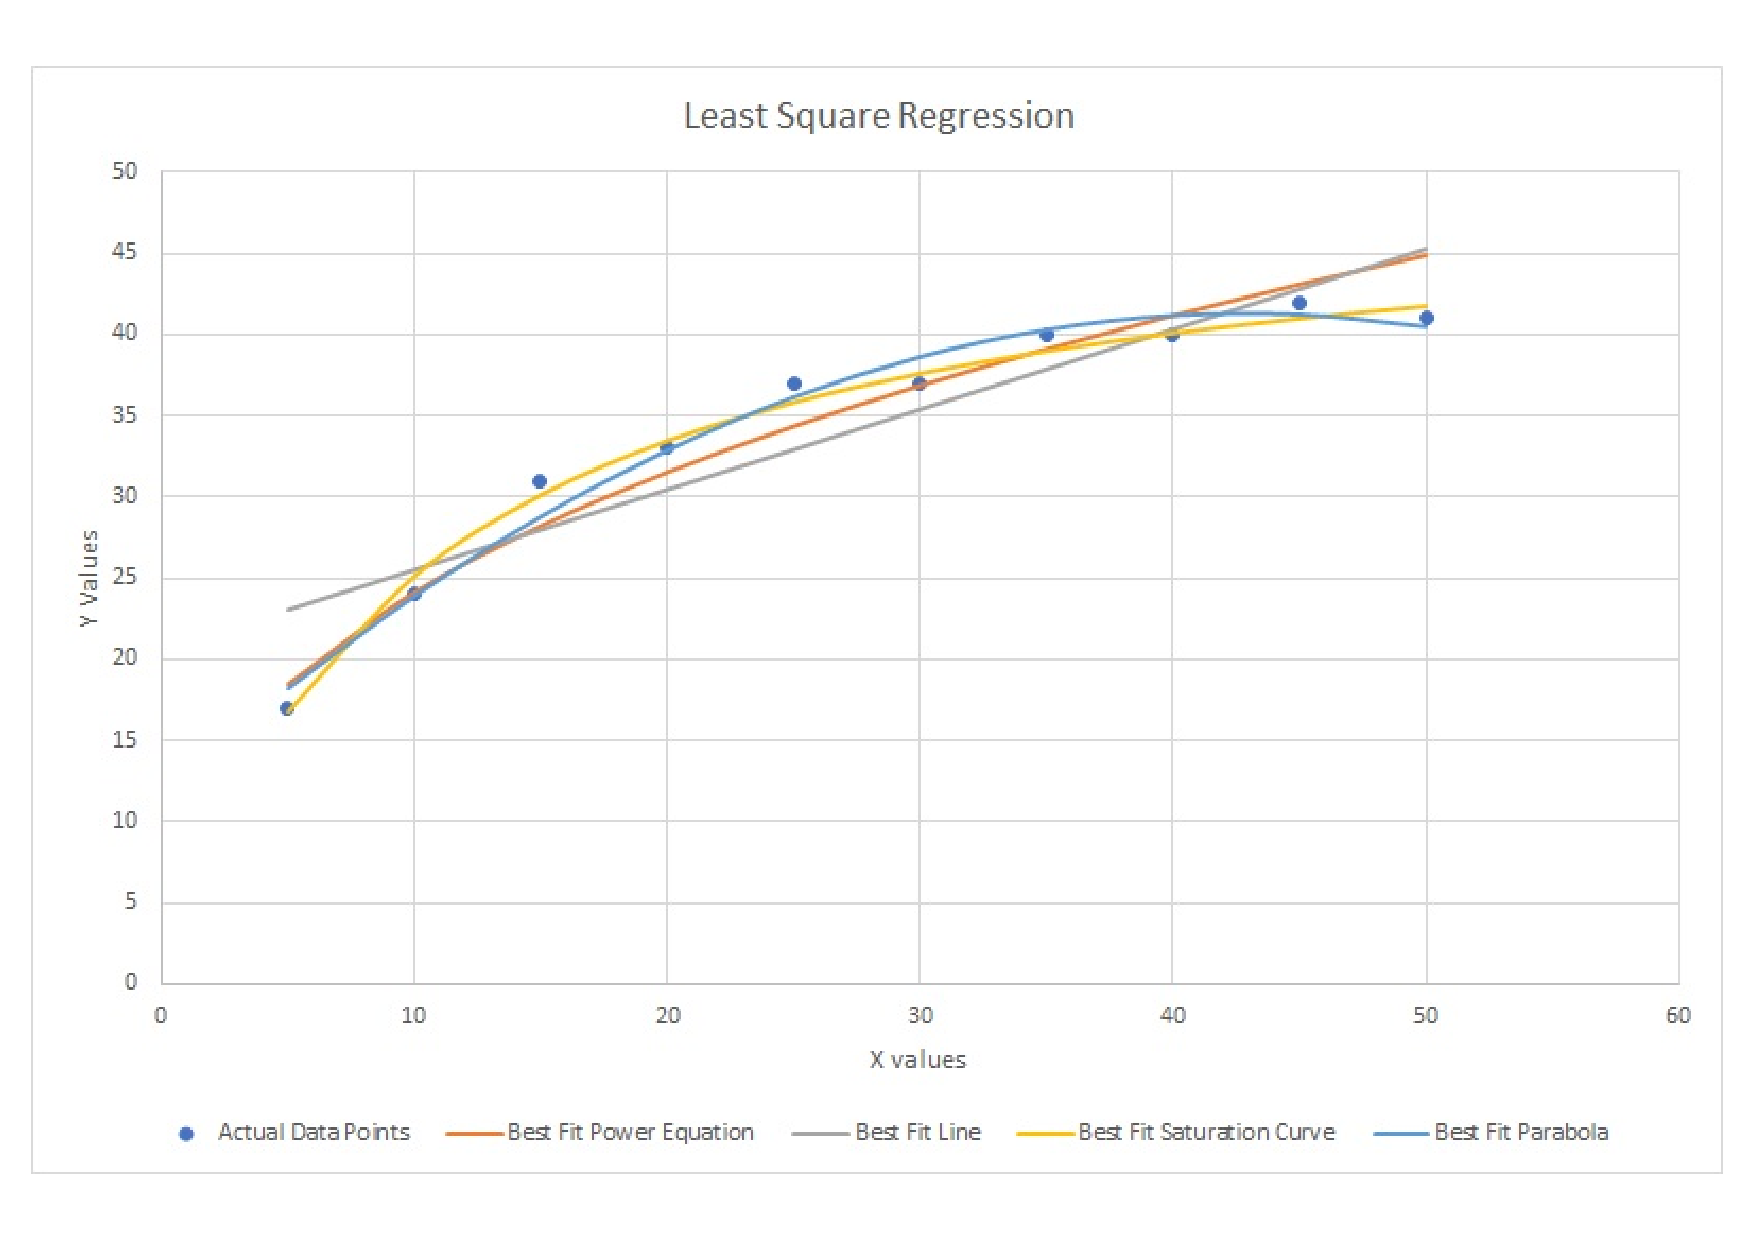
\includegraphics[width=0.9\textwidth]{A5P2Graph.pdf} 
  	\caption{Best Fit Curves plotted using Least Square Regression.}
  	\label{fig:q12} 
\end{figure}

\begin{table}[!htb]
    \caption{Best Fit Type vs $r^2$ values}
    \centering
    \renewcommand{\arraystretch}{1.5}
    \begin{tabular}{ccc}
    \toprule
    \textbf{Best Fit Type}& \textbf{Equation}& \textbf{Coefficient of Determination $r^2$}   \\
    \midrule
         Straight Line & $y = 20.6 + 0.494545x $& 0.838491 \\
         Power Equation & $y = 9.952915 x ^{0.385077}$ & 0.9377 \\
         Saturation Curve & $y= \frac{50.092118x}{9.891369 + x} $ & 0.989190\\
         Parabola & $ y = 11.766667 + 1.377879x - 0.016061x^2$ & 0.979983 \\
    \bottomrule
    \end{tabular}
    \label{tab:tab2}
\end{table}

%%%%%%%%%%%%%%%%%%%%%%%%%%%%%%%%%%%%%%%%%%%%%%%%%%%%%%

\subsection{Inferences}
I deduce the following inferences from this problem:
\begin{itemize}
    \item [1] For regression, the best fit is determined from the value of $r^2$, the more closer $r^2$ is to 1, the better the fit is. As apparent from Table ~\ref{tab:tab2}, the $r^2$ values follow the trend :\\
    \begin{center}
        0 < Line < Power Equation < Parabola < Saturation Curve < 1
    \end{center}
    \item [2] The linear fit is obviously inadequate. This can also be supported from its lower $r^2$ value of 0.838491. Moreover, the best fit line does not pass through most of the points. 
    \item [3] Although the power equation follows the general trend of data, it is also inadequate due to the following reasons 
    \begin{itemize}
        \item [a] Its $r^2$ value is low when compared to the Saturation curve and parabolic fit.
        \item [b] The power equation also does not pass through most of the points. Thus, we expect its standard error to be high.
     \end{itemize}
     \item [4] The parabolic fit seems to represent the given data points quite satisfactorily with a $r^2$ value of 0.98. However, the parabolic fit has a lower $r^2$ value when compared to the saturation curve. 
     \item [5] The saturation curve best fits the given data points with the largest $r^2$ value of 0.989190. We can apparently see that the data points are scattered around the saturation curve and the parabolic fit, yet the saturation curve seems to be a closer fit with a lesser standard error as seen visually. 
     \item [6] Although the difference is probably not statistically significant, in the absence of additional information, \textbf{we can conclude that the saturation curve best fits the given data. }
     \item [7] Errors could be propagated due to taking 
     \begin{itemize}
         \item [a] Logarithm in evaluating Power Equation
         \item [b] Reciprocal in evaluating Saturation Curve
     \end{itemize}
     \item [8] From the above inference, we can also conclude that any data point must not be zero for evaluating power equation and saturation curve which seems quite obvious as well. 
     \item [9] If it is required that a line needs to pass through the given points, we could use a technique popularly called as \href{https://en.wikipedia.org/wiki/Interpolation}{Interpolation} which ensures that the given curve passes through the given data points.
     \item [10] Last but not the least, the obtained system of linear equations must not be ill-conditioned or singular as we use Gaussian Elimination to obtain the solution of the same. 
\end{itemize}

%%%%%%%%%%%%%%%%%%%%%%%%%%%%%%%%%%%%%%%%%%%%%%%%%%%%%%

\subsection{Code}
The code used in Problem 3 is mentioned in Listing~\ref{listing:5} and Listing ~\ref{listing:6}

\inputminted[breaklines,
 mathescape,
 linenos,
 numbersep=5pt,
 frame=single,
 numbersep=5pt,
 xleftmargin=0pt]{c}{A5P2L.c}
 \captionof{listing}{Code snippet used in the Problem of Regression (Line, Power Equation, Saturation Curve).}
\label{listing:5}

\inputminted[breaklines,
 mathescape,
 linenos,
 numbersep=5pt,
 frame=single,
 numbersep=5pt,
 xleftmargin=0pt]{c}{A5P2P.c}
 \captionof{listing}{Code snippet used in the Problem of Regression (Parabola).}
\label{listing:6}


%%%%%%%%%%%%%%%%%%%%%%%%%%%%%%%%%%%%%%%%%%%%%%%%%%%%%%

\subsection{Contributions}
In the above problem, \textit{my original contributions} are - 
\begin{itemize}
    \item Designing of the Algorithm and Code
    \item Tabulation of Results
    \item Plotting the graphs on MS Excel
    \item Drawing conclusions by looking at the Results obtained.
    \item Writing the report in LaTeX. 
\end{itemize}

%%%%%%%%%%%%%%%%%%%%%%%%%%%%%%%%%%%%%%%%%%%%%%%%%%%%%%

\subsection{Alternate Methods}
\begin{itemize}
    \item [1] In the limit of more data points, the result obtained could differ. This is because we work on minimizing the sum of squares of error terms which could decrease for a certain fit as compared to another fit for larger number of data points.
    \item [2] It can also be brought out to light that we could not only regress the given data using a quadratic best fit, but also try out a cubic best fit and so on.
    \item [3] \href{https://en.wikipedia.org/wiki/Spline_interpolation}{Spline Interpolation} is a technique that ensures that the resultant curve obtained post interpolation passes through the given data points.
    \item [4] We could also exploit the \href{https://en.wikipedia.org/wiki/Lagrange_polynomial}{Lagrange Interpolation} to find out the curve that passes through the given set of points.
    \item [5] In an ill-conditioned system, we would require an alternative approach, preferably the LU Decomposition Algorithm or Gauss-Siedel Method, which ever suits the given data. 
    \item [6] In case of Singular systems we would require to throw an exception that the given data points are inaccurate. However, this happens in the rarest of rare cases.
    \item [7] As it seems quite obvious, that given the nature of the function for the data points, it will be much more easier computing the best fit rather than comparing among different categories.
\end{itemize}

\newpage
\section{Problem 3}
Dynamic viscosity of water $\mu$ (10$^{-3}$ N·s/m2) is related to
temperature T (°C) in the following manner:
\begin{table}[h!]
\begin{center}
    \label{tab:table1}
    \begin{tabular}{l |l l l l l l}
    %\hline
      T & 0 & 5 & 10 & 20 & 30 & 40 \\
      \hline
      \mu & 1.787 & 1.519 & 1.307 & 1.002 & 0.7975 & 0.6529
      %\hline
    \end{tabular}
\end{center}
\end{table}
\begin{itemize}
  \item [(a)] Use the Newton divided difference interpolation to predict $\mu$ at $T$ = 7.5$^{\circ}$C.
    \item [(b)] Use polynomial regression to fit a parabola to data in order to make the same prediction.
     \item [(c)] Plot the data as discrete points and show both the interpolation and the regression lines in the same set of axes. What is your inference ?
\end{itemize}

\subsection{Approach}

In this problem, I shall use the Least-Square Regression to find out the best-fit parabola for a given set of data points. I shall also interpolate the data to find the fifth-degree polynomial passing through the six data points given. 

%%%%%%%%%%%%%%%%%%%%%%%%%%%%%%%%%%%%%%%%%%%%%%%%%%%%%%

\subsection{Algorithm}
In this section, I present the pseudocode/flowchart of the algorithm used to solve the problem.

The pseudocode for the summation is provided in Algorithm~\ref{alg3} and ~\ref{alg5}

\begin{center}
\begin{algorithm}[H]\label{alg3}

\SetAlgoLined{
n $\gets$ 6 \\
x $\gets$ [$x_0,x_1,x_2.....x_{5}$] \\
y $\gets$ [$y_0,y_1,y_2.....y_{5}$] \\
\For{$j=0$ to n-1}{
  \For{$i=n-1$ to j}{
     $y_i$ $\gets$ $\frac{y_i-y_{i-1}}{x_i-x_{i-j-1}}$ \\
  }
}
\For{$i=n-1$ to 0}{
   m $\gets$ 1 \\
   \For{$j=0$ to i}{
      m $\gets$ m*(7.5-$x_j$)\\
   }
   m $\gets$ m * $y_j$\\
   sum $\gets$ sum + m \\
}
}
\caption{Interpolation}
\end{algorithm}    
\end{center}
\begin{center}
\begin{algorithm}[H]\label{alg5}
\SetAlgoLined
{
n $\gets$ 6 \\
x $\gets$ [$x_0,x_1,x_2.....x_{5}$] \\
y $\gets$ [$y_0,y_1,y_2.....y_{5}$] \\
$s$ $\gets$ n \\
$s_x$ $\gets$ 0 \\ 
$s_y$ $\gets$ 0 \\ 
$s_{xy}$ $\gets$ 0 \\ 
$s_{xx}$ $\gets$ 0 \\ 
$s_{xxy}$ $\gets$ 0 \\
$s_{xxx}$ $\gets$ 0 \\
$s_{xxxx}$ $\gets$ 0 \\
$s_t$ $\gets$ 0 \\
$s_r$ $\gets$ 0 \\
\For {$i=0$ to n-1}{
  $s_x$ $\gets$ $s_x + x_i$ \\ 
  $s_y$ $\gets$ $s_y + y_i$ \\
  $s_{xy}$ $\gets$ $s_{xy} + x_iy_i$ \\
  $s_{xx}$ $\gets$ $s_{xx} + x_ix_i$ \\
  $s_{xxy}$ $\gets$ $s_{xxy} + x_ix_iy_i$ \\
  $s_{xxx}$ $\gets$ $s_{xxx} + x_ix_ix_i$ \\
  $s_{xxxx}$ $\gets$ $s_{xxxx} + x_ix_ix_ix_i$ \\
}
A $\gets$
$\begin{pmatrix}
s & s_x & s_{xx}\\
s_x & s_{xx} & s_{xxx} \\
s_{xx} & s_{xxx} & s_{xxxx}
\end{pmatrix}$ \\
B $\gets$
$\begin{pmatrix}
s_y \\
s_{xy} \\
s_{xxy}
\end{pmatrix}$ \\
X $\gets$
$\begin{pmatrix}
a_0 \\
a_1 \\
a_2
\end{pmatrix}$ \\
Solve AX = B using Gauss Elimination \textbf{Assignment 4}\\
mean $\gets$ $\frac{s_y}{n}$ \\
\For{$i=0$ to n-1}{
   $s_r$ $\gets$ $s_r$ + $(y_i-a_0-a_1x_i-a_2{x_i}^2)^2$ \\
   $s_t$ $\gets$ $s_t$ + $(y_i-mean)$ 
}
$r^2$ $\gets$ $\frac{s_t-s_r}{s_t}$\\
$r$ $\gets$ $\sqrt{\frac{s_t-s_r}{s_t}}$\\
}
 \caption{Least Square Regression}
\end{algorithm}    
\end{center}

%%%%%%%%%%%%%%%%%%%%%%%%%%%%%%%%%%%%%%%%%%%%%%%%%%%%%%
\subsection{Results}

In this section, I shall plot the graphs that provide an overview of my findings during this problem. 

I shall plot the graphs showing the best fit parabola for a given set of data points and also plot the data points given as discrete points  in Figure~\ref{fig:q13}.The interpolated polynomial is also shown in the same graph. The results are also summarized below. 

The value of $\mu$ in ($10^{-3}$ N-s/$m^2$) at T = $7.5^{\circ}$C obtained using
\begin{itemize}
    \item [1] Interpolation is 1.406863
    \item [2] Parabolic Best Fit is 1.426889
\end{itemize}

\begin{figure}[!tbh]
  	\centering
  	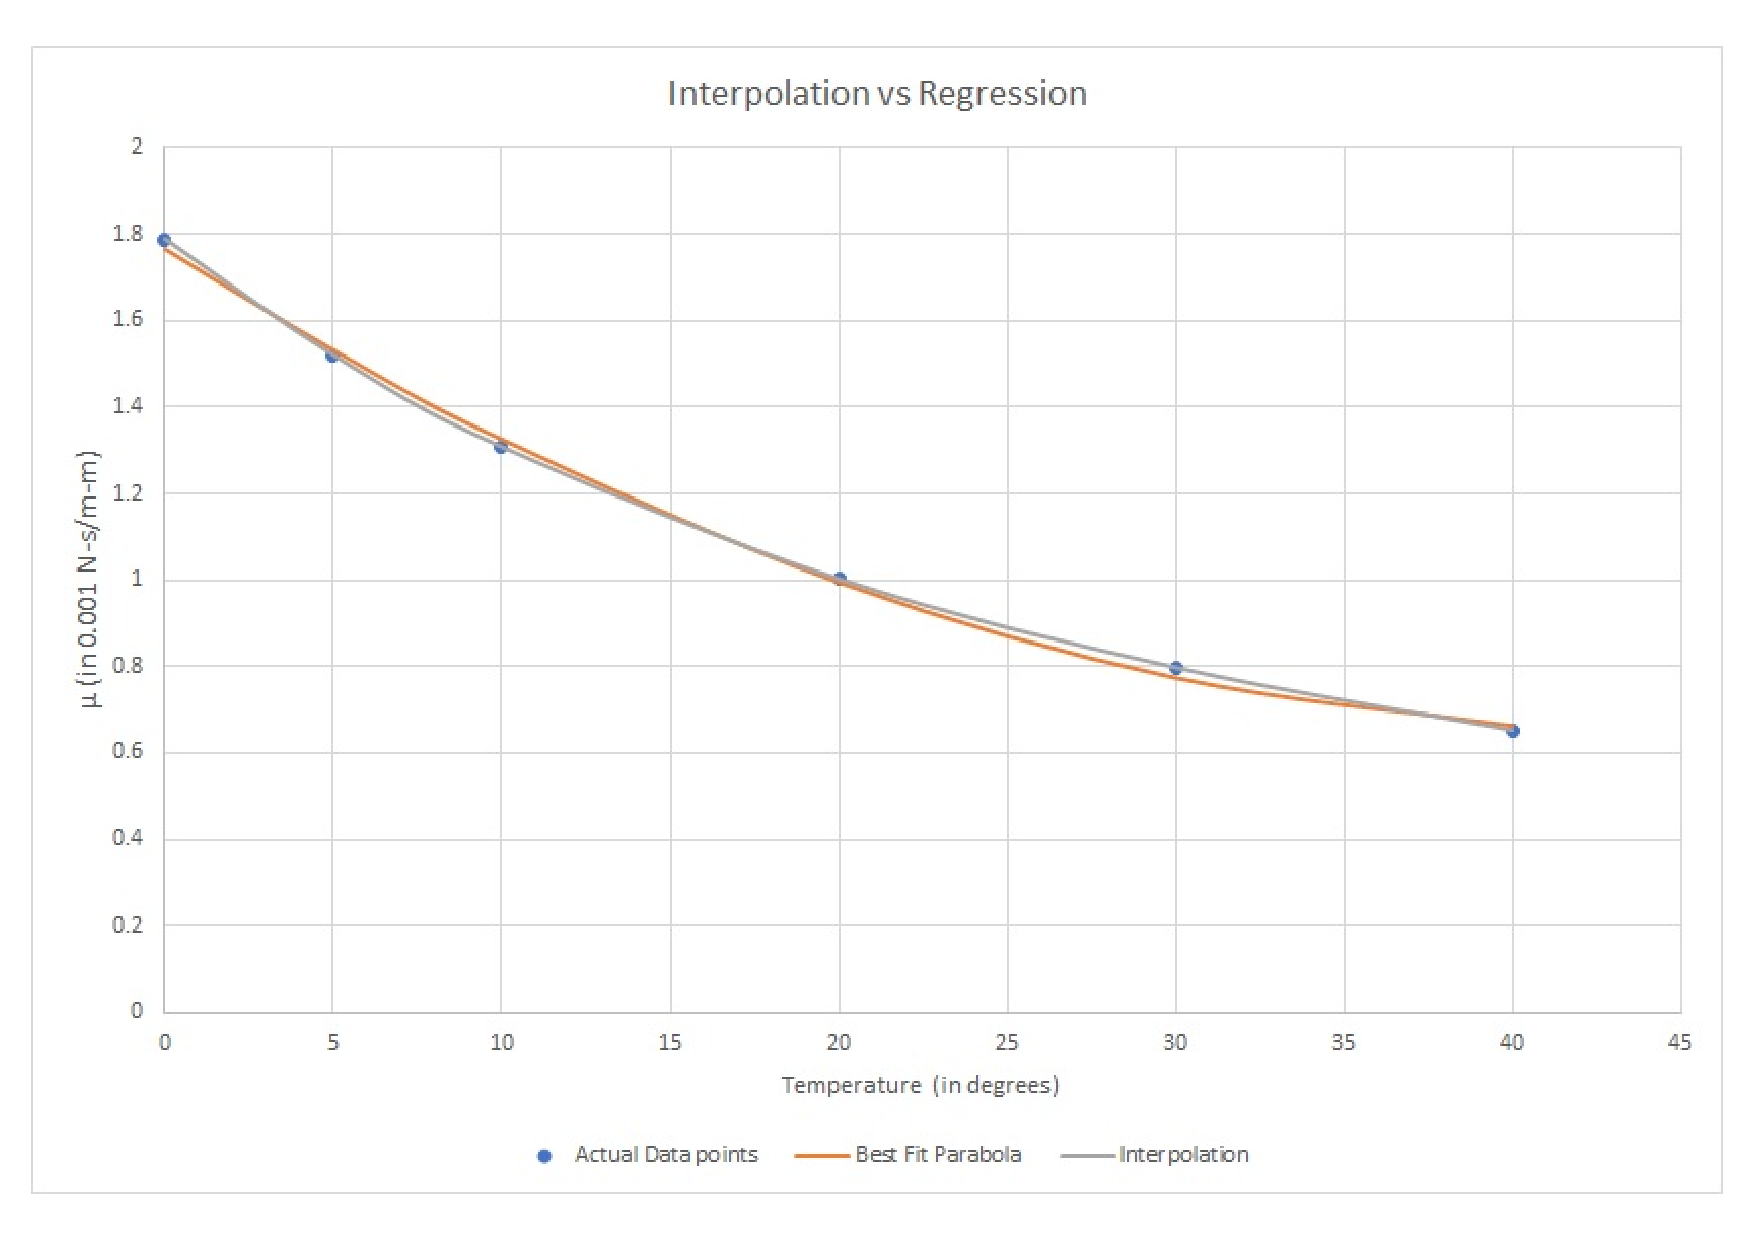
\includegraphics[width=0.9\textwidth]{A5P3Graph.pdf} 
  	\caption{Best Fit Parabola vs Interpolated fifth order equation}
  	\label{fig:q13} 
\end{figure}


%%%%%%%%%%%%%%%%%%%%%%%%%%%%%%%%%%%%%%%%%%%%%%%%%%%%%%

\subsection{Inferences}
I deduce the following inferences from this problem:
\begin{itemize}
    \item [1] The working rule of Interpolation is that the interpolated curve passes through the given set of data points; whereas the working rule of Regression is to minimize the error. The two algorithms thus, greatly differ in their approach to the same problem.
    \item [2] As apparent, the interpolated line passes through all the given six data points whereas the best fit parabola seldom passes through the given data points. 
    \item [3] The value of $r^2$ for the parabolic fit is 0.998282 which is very close to 1, thus represents the data points very closely.
    \item [4] Since interpolated curve passes through all the given data points, it may seem quite absurd at first sight that we associate an error with the same. Yes, this is rather true and we use an alternate definition of error in interpolation of a polynomial. 
    \item [5] The error in interpolation of a polynomial can be obtained using an analog to Taylor's Theorem in the following manner 
    \begin{equation}
    R_n(x) = \frac{f^{n+1}(c)}{n+1} (x-x_0)(x-x_1)(x-x_2)...(x-x_n) 
    \end{equation}
    \item [6] Here we have used the fact that the interpolation of 6 data points would be a polynomial of degree 5. We could also interpolate the given data using a quadratic function or a cubic function which is often termed as \href{https://en.wikipedia.org/wiki/Spline_interpolation}{Spline Interpolation}
    \item [7] The predictions made using Interpolation and Regression arer listed below again. \\
    The value of $\mu$ in ($10^{-3}$ N-s/$m^2$) at T = $7.5^{\circ}$C obtained using
  \begin{itemize}
    \item [1] Interpolation is 1.406863
    \item [2] Parabolic Best Fit is 1.426889
  \end{itemize}
  \item [8] It may not quite seem obvious as to which of the two points is closer to the real value at T=$7.5^{\circ}C$. This can be determined only experimentally. However, it is generally assumed that interpolation would give a closer result than the least square regression.
  \item [9] It may seem quite contradictory at first sight that we use both Interpolation and Regression on the same data. This is because Interpolation assumes that the given data is exact, that is, there is no error associated with it. However, Regression assumes that the given data has a certain finite error associated with it. It is strange that once we assume that data is perfect and the other time we assume that it is imperfect.
  \item [10] To actually decide which is better - Interpolation or Regression ? - It actually depends on whether we know the given form of data. If we know already that the given form of data is of a power equation, we could use least square regression to obtain the power equation which would suit the data better than interpolation. 
  \item [11] In the Code for Regression, we have used Gaussian Elimination which otherwise fails when the system of equations is Singular or Ill-Conditioned. We need to check for the same before running the Code. 
\end{itemize}

%%%%%%%%%%%%%%%%%%%%%%%%%%%%%%%%%%%%%%%%%%%%%%%%%%%%%%

\subsection{Code}
The code used in Problem 3 is mentioned in Listing~\ref{listing:7} and Listing ~\ref{listing:8}

\textbf{Note :} The y values have been rescaled and taken in $10^{-3}$ units in both the codes. 

\inputminted[breaklines,
 mathescape,
 linenos,
 numbersep=5pt,
 frame=single,
 numbersep=5pt,
 xleftmargin=0pt]{c}{A5P3I.c}
 \captionof{listing}{Code snippet used in the Problem of Interpolation.}
\label{listing:7}

\inputminted[breaklines,
 mathescape,
 linenos,
 numbersep=5pt,
 frame=single,
 numbersep=5pt,
 xleftmargin=0pt]{c}{A5P3P.c}
 \captionof{listing}{Code snippet used in the Problem of Regression.}
\label{listing:8}

%%%%%%%%%%%%%%%%%%%%%%%%%%%%%%%%%%%%%%%%%%%%%%%%%%%%%%

\subsection{Contributions}
In the above problem, \textit{my original contributions} are - 
\begin{itemize}
    \item Designing of the Algorithm and Code
    \item Tabulation of Results
    \item Plotting the graphs on MS Excel
    \item Drawing conclusions by looking at the Results obtained.
    \item Writing the report in LaTeX. 
\end{itemize}
%%%%%%%%%%%%%%%%%%%%%%%%%%%%%%%%%%%%%%%%%%%%%%%%%%%%%%

\subsection{Alternate Methods}
\begin{itemize}
    \item [1] As mentioned earlier, the working rules of Interpolation and Regression are completely different and cannot be judged on a fair basis.
    \item [2] Given the nature of the plot and data points, it will be convenient to find out which is a better approximation - Interpolation or Regression, which otherwise cannot be compared in my opinion.
    \item [3] Rather than obtaining a fifth order polynomial equation, we could obtain a second order of third order polynomial equation using Spline Interpolation. 
    \item [4] \href{https://en.wikipedia.org/wiki/Lagrange_polynomial}{The Lagrange Polynomial} is also a good technique of interpolation. 
    \item [5] Besides from the techniques mentioned in the Problem Sheet, there are several other methods also to find the best fit for a given set of data points. Some of the common ones are \href{https://en.wikipedia.org/wiki/Function_approximation}{Function Approximation} and \href{https://en.wikipedia.org/wiki/Smoothing}{Smoothing.}
\end{itemize}
\end{document}
